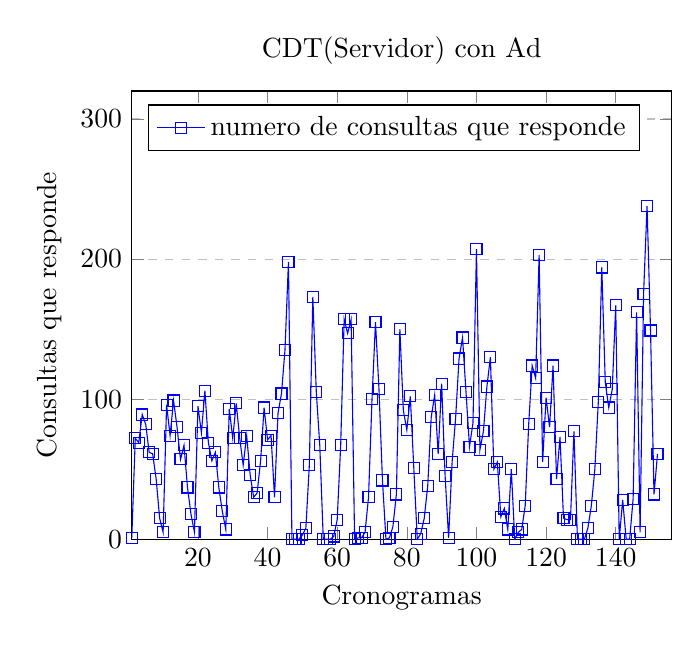
\begin{tikzpicture}
\begin{axis}[
    %CDT = carga de trabajo
    %AEPxT = Algoritmo DETRMINISTA
    title={CDT(Servidor) con Ad},
    xlabel={Cronogramas},
    ylabel={Consultas que responde},
    xmin=1, xmax=156,
    ymin=0, ymax=320,
    xtick={},
    ytick={},
    legend pos=north west,
    ymajorgrids=true,
    grid style=dashed,
]

\addplot[
    color=blue,
    mark=square,
    ]
    coordinates {
   %CARGA DE TRABAJO Servidor
(1,1)
(2,72)
(3,69)
(4,89)
(5,82)
(6,62)
(7,61)
(8,43)
(9,15)
(10,5)
(11,96)
(12,74)
(13,99)
(14,80)
(15,57)
(16,67)
(17,37)
(18,18)
(19,5)
(20,95)
(21,76)
(22,106)
(23,69)
(24,56)
(25,62)
(26,37)
(27,20)
(28,7)
(29,93)
(30,72)
(31,97)
(32,72)
(33,53)
(34,74)
(35,46)
(36,30)
(37,33)
(38,56)
(39,94)
(40,71)
(41,74)
(42,30)
(43,90)
(44,104)
(45,135)
(46,198)
(47,0)
(48,0)
(49,0)
(50,3)
(51,8)
(52,53)
(53,173)
(54,105)
(55,67)
(56,0)
(57,0)
(58,0)
(59,2)
(60,14)
(61,67)
(62,157)
(63,147)
(64,157)
(65,0)
(66,1)
(67,1)
(68,5)
(69,30)
(70,100)
(71,155)
(72,107)
(73,42)
(74,0)
(75,1)
(76,9)
(77,32)
(78,150)
(79,92)
(80,78)
(81,102)
(82,51)
(83,0)
(84,4)
(85,15)
(86,38)
(87,87)
(88,103)
(89,61)
(90,111)
(91,45)
(92,1)
(93,55)
(94,86)
(95,129)
(96,144)
(97,105)
(98,66)
(99,83)
(100,207)
(101,64)
(102,77)
(103,109)
(104,130)
(105,50)
(106,55)
(107,16)
(108,22)
(109,7)
(110,50)
(111,0)
(112,5)
(113,7)
(114,24)
(115,82)
(116,124)
(117,115)
(118,203)
(119,55)
(120,101)
(121,80)
(122,124)
(123,43)
(124,73)
(125,15)
(126,14)
(127,14)
(128,77)
(129,0)
(130,0)
(131,0)
(132,8)
(133,24)
(134,50)
(135,98)
(136,194)
(137,112)
(138,94)
(139,107)
(140,167)
(141,0)
(142,28)
(143,0)
(144,0)
(145,29)
(146,162)
(147,5)
(148,175)
(149,238)
(150,149)
(151,32)
(152,61)
    };
    \legend{numero de consultas que responde}

\end{axis}
\end{tikzpicture}
